\documentclass{beamer}
\usepackage{graphicx}
\usepackage{algorithm2e}
\usepackage{amsmath,amssymb}
\usepackage{color, colortbl}

%%% Beamer Theme %%%
\usetheme{JuanLesPins}
\usecolortheme{beaver}
\beamertemplatenavigationsymbolsempty
\renewcommand\mathfamilydefault{\rmdefault}
%%%

\setlength{\parindent}{0.0cm}

\date{12 March 2012}
\author{Jeremy Mayeres, Charles Newton, Peter Tonner}
\title{Facilitating Large-Scale Graph Searches with Lock-Free Pairing Heaps}

\begin{document}
\maketitle

\begin{frame}{Project Overiew}
  \begin{itemize}
    \item We are constructing a lock-free version of a Pairing heap (a self-balancing heap.)
    \item Pairing heaps have an efficient \texttt{decreaseKey} implementation
      (near-constant performance) that allow you to decrease the value in a heap without
      reinserting it.
    \item This improves the asymptotic performance of certain algorithms (e.g., Dijkstra's algorithm.)
    \item We are comparing our heap against Skipqueues (a priority queue backed with a Skiplist.)
  \end{itemize}
\end{frame}

\begin{frame}{Dijkstra's Algorithm}
  \begin{block}{Single-Source Shortest Path Problem}
    In a weighted graph $G=(V,E)$, find the shortest path from a target
    vertex $v \in V$ to all other vertices in the graph.
  \end{block}
  \begin{itemize}
    \item Push every node in a graph into a priority queue (PQ.) In the PQ, 
      each node is weighted by current information we have about their distance.
    \item Initially, all nodes have a distance of $\infty$, except the target
      node, which has a distance of $0$.
    \item Dynamic programming approach: Inductively build up our shortest routes.
      \begin{itemize}
        \item Pop off the node on the PQ with the smallest distance. (The shortest path from the source to this
          node is finished.)
        \item Update the weights in the PQ with the distances emanating from the popped node.
      \end{itemize}
    \end{itemize}
\end{frame}

\begin{frame}{Skiplists}
  \begin{itemize}
    \item Skiplists are constructed from a hierarchy of linked lists with the \textit{Skiplist property}:
      the set of elements contained in level $i$ is a subset of all the levels below it.
    \item Links allow you to do a binary search and ``jump'' around a list.
    \item The height of an element is randomly sampled from a power-law distribution: the probability of
      a node having a height of $i \geq 0$ is $2^{-i}$.
    \item Time complexity of operations are probabilistically the same as for a binary search tree, but
      $\mathcal{O}(n)$ in the worst case.
  \end{itemize}
  \begin{center}
    \includegraphics[scale=0.75]{img/skiplist-crop.pdf}
  \end{center}
\end{frame}

\begin{frame}{Skiplists (Search)}
  \begin{itemize}
    \item For each level, move right until you run into a node greater than your target. Then, from
      this point, move right on the next lowest level, and repeat.
    \item Likely runs in $\mathcal{O}(\log n)$ time.
    \item Head / tail nodes have values of $-\infty$ and $\infty$, respectively.
  \end{itemize}
  \begin{center}
    \includegraphics[scale=0.75]{img/skiplistSearch15-crop.pdf}
  \end{center}
\end{frame}

\begin{frame}{Next and Previous Windows}
  \begin{itemize}
    \item A useful abstraction to make is the set of all pointers
      related to a given node. (Aggregate all the pointers related to one node.)
    \item $\mathtt{prev[}i\mathtt{]} \rightarrow$ the node in level $i$ pointing to the target node.
    \item $\mathtt{next[}i\mathtt{]} \rightarrow$ the node the target node points to at level $i$.
    \item Use the search process to construct these sets.
  \end{itemize}
  \begin{center}
    \includegraphics[scale=0.75]{img/skiplistInsert5-crop.pdf}
  \end{center}
\end{frame}

\begin{frame}{Skiplists (Insertion)}
  \begin{itemize}
    \item Insertion: Find the location the target should be at.
      Set all of the node's next pointers to $\mathtt{next[}i\mathtt{]}$ and set
      the next pointers at each $\mathtt{prev[}i\mathtt{]}$ to the new node.
  \end{itemize}
  \begin{center}
    \includegraphics[scale=0.75]{img/skiplistSearch15-crop.pdf}
  \end{center}
  \begin{center}
    \includegraphics[scale=0.75]{img/skiplistInsert5-crop.pdf}
  \end{center}
\end{frame}

\begin{frame}{Skiplists (Deletion)}
  \begin{itemize}
    \item Deletion: Set all of the next pointers in $\mathtt{prev[}i\mathtt{]}$ 
      equal to $\mathtt{next[}i\mathtt{]}$.
  \end{itemize}
  \begin{center}
    \includegraphics[scale=0.75]{img/skiplistSearch15-crop.pdf}
  \end{center}
  \begin{center}
    \includegraphics[scale=0.75]{img/skiplistInsert5-crop.pdf}
  \end{center}
\end{frame}

\begin{frame}{Lock-free Skiplists}
  \begin{itemize}
    \item Instead of linked lists at each level, we use lock-free linked lists.
    \item We lose the Skiplist property. (Levels aren't necessarily subsets of each other.) In particular,
      this means we need to always verify a node is in the lowest level.
  \end{itemize}
\end{frame}

\begin{frame}{Lock-free Skiplists}
  \begin{itemize}
    \item Instead of linked lists at each level, we use lock-free linked lists.
    \item Linearization point: membership is defined at the lowest level of the Skiplist.
    \item We lose the Skiplist property. (Levels aren't necessarily subsets of each other.) In particular,
      this means we need to always verify a node is in the lowest level.
  \end{itemize}
\end{frame}

\begin{frame}{Lock-Free Skiplists (Insertion)}
  \begin{itemize}
    \item Construct the $\mathtt{prev[}i\mathtt{]}$ and $\mathtt{next[}i\mathtt{]}$ sets.
    \item Set all of the node's next pointers to $\mathtt{next[}i\mathtt{]}$.
    \item If we can CAS the node into the bottom level, continue. Otherwise, something changed, and
      restart (reconstruct $\mathtt{prev[}i\mathtt{]}$ and $\mathtt{next[}i\mathtt{]}$).
    \item Next, CAS all $\mathtt{prev[}i\mathtt{]}$ to the new node. If a CAS fails, reconstruct
      $\mathtt{prev[}i\mathtt{]}$.
  \end{itemize}
\end{frame}

\begin{frame}{Lock-Free Skiplists (Deletion)}
  \begin{itemize}
    \item Pointers are atomically \textit{markable}.
      \begin{itemize}
        \item In C / C++, steal a bit from the pointer.
        \item In Java, use \texttt{AtomicMarkableReference}.
      \end{itemize}
    \item Construct the $\mathtt{prev[}i\mathtt{]}$ and $\mathtt{next[}i\mathtt{]}$ sets.
    \item For each pointer in our target node, mark them as deleted.
  \end{itemize}
\end{frame}

\begin{frame}{Optimized \texttt{decreaseKey} for Lock-Free Skiplists}
  \begin{itemize}
    \item Currently, to implement a \texttt{decreaseKey} for Skiplists, we need to
      do two $\mathcal{O}(\log n)$ operations (one insert and one delete.)
    \item We can optimize this in some cases by removing redundant work: reuse the
      $\mathtt{prev[}i\mathtt{]}$ set as a starting point for the next insertion.
  \end{itemize}
\end{frame}

\begin{frame}{Pairing Heaps}
  \begin{itemize}
    \item Pairing Heaps were introduced by Fredman and Tarjan.
      \item \texttt{decreaseKey} runs in $2^{\mathcal{O}(\sqrt{\log \log n})}$
        time
        \begin{itemize}
          \item In practice, constant time. E.g., for a graph with a billion nodes,
            $2^\sqrt{\log \log 10^9} = 3.34$.
        \end{itemize}
        
  \end{itemize}
\end{frame}

\begin{frame}{Pairing Heaps: Melding Two Heaps}
  \includegraphics[scale=1.0]{img/meld.png}
\end{frame}

\begin{frame}{Pairing Heaps: \texttt{deleteMin}}
  \begin{itemize}
    \item Pairing heaps have a two-step deleteMin operator.
  \end{itemize}
  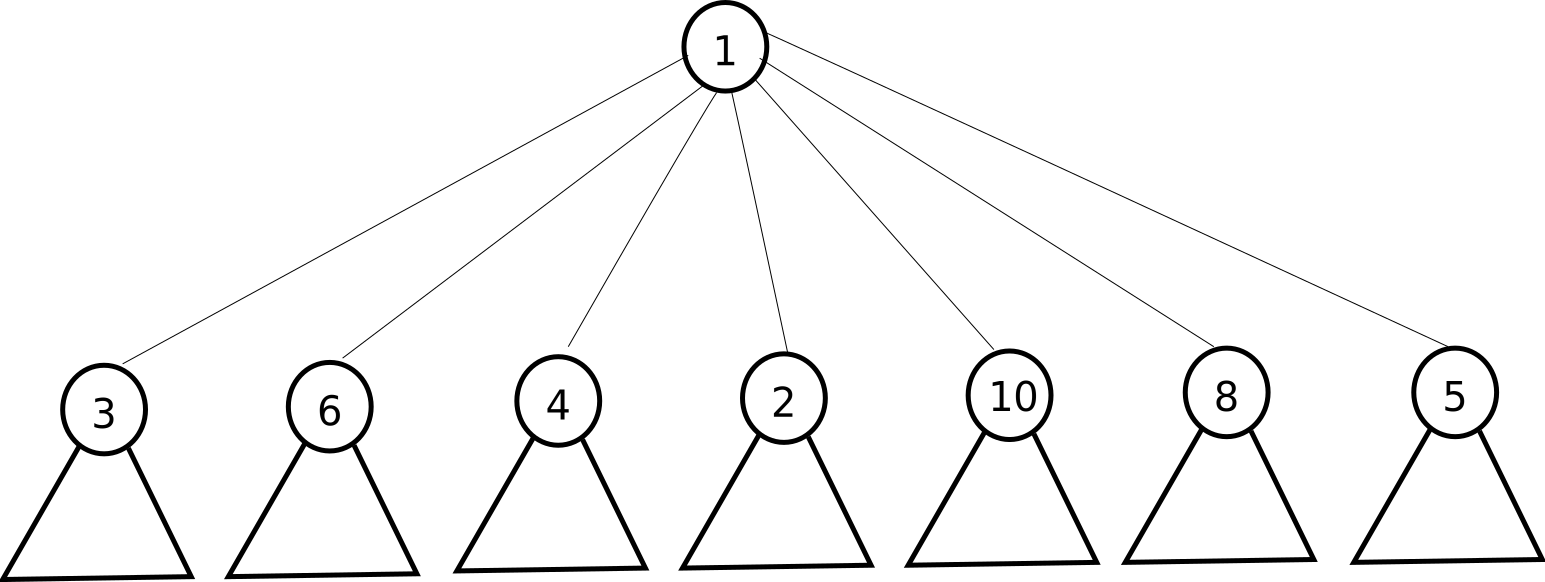
\includegraphics[scale=1.0]{img/deleteMin1.png}
\end{frame}

\begin{frame}{Pairing Heaps: \texttt{deleteMin}}
  \begin{itemize}
    \item After removing the root, \texttt{meld} each pair of heaps.
  \end{itemize}
  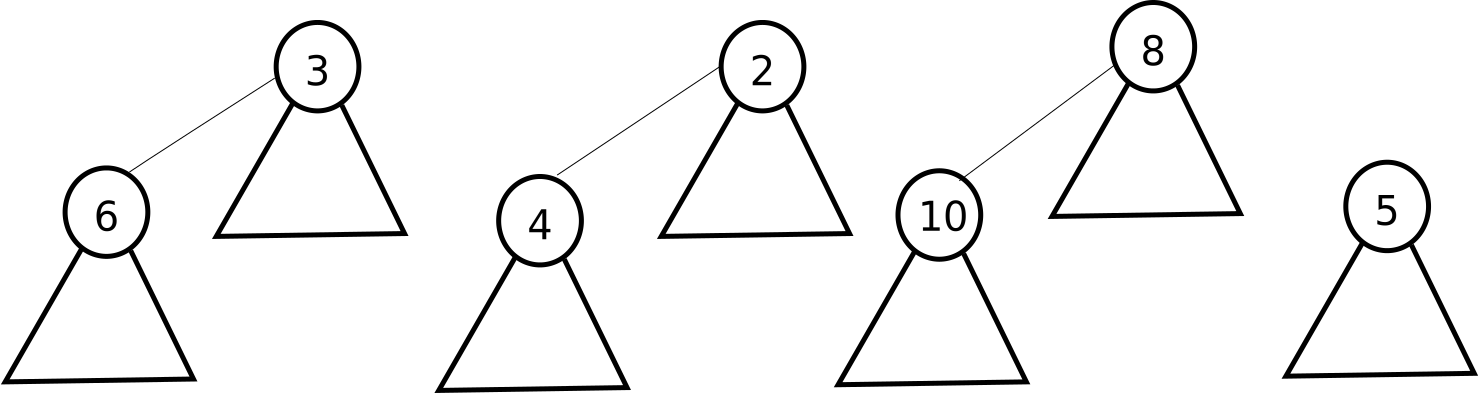
\includegraphics[scale=1.0]{img/deleteMin2.png}
\end{frame}

\begin{frame}{Pairing Heaps: \texttt{deleteMin}}
  \begin{itemize}
    \item \texttt{meld} each resultant heap from right-to-left.
  \end{itemize}
  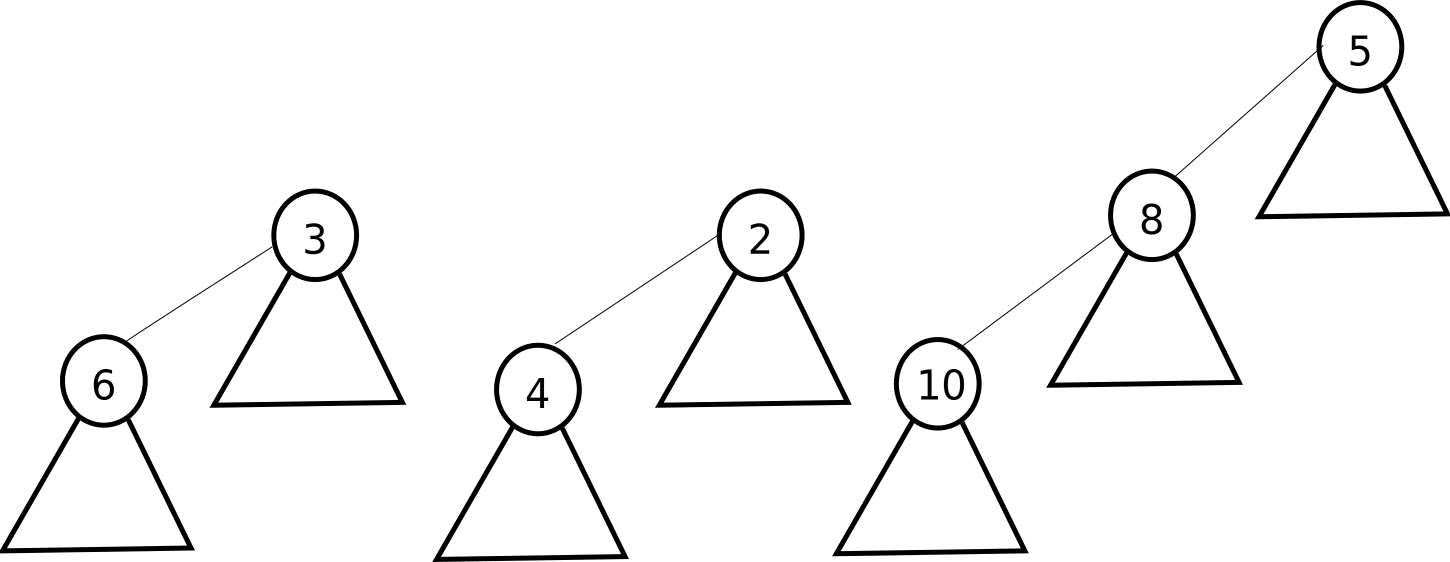
\includegraphics[scale=1.0]{img/deleteMin3.png}
\end{frame}

\end{document}
